\documentclass{ltxdoc}
\usepackage[T1]{fontenc}
\usepackage{lmodern}
\usepackage{morefloats}
\usepackage{tikz}
\usepackage{braids}
\usetikzlibrary{
  braids,
  decorations.markings
}
\usepackage[numbered]{hypdoc}
\definecolor{lstbgcolor}{rgb}{0.9,0.9,0.9} 
 
\usepackage{listings}
\lstloadlanguages{[LaTeX]TeX}
 \lstset{
  gobble=2,
  breakatwhitespace=true,
  breaklines=true,
  language=[LaTeX]TeX,
  basicstyle=\small\ttfamily,
  keepspaces=true,
  columns=fullflexible
}
 
\usepackage{fancyvrb}

\newenvironment{example}
{\VerbatimEnvironment
  \begin{VerbatimOut}{example.out}}
{\end{VerbatimOut}
  \begin{center}
  \setlength{\parindent}{0pt}
  \fbox{\begin{minipage}{.9\linewidth}
    \lstinputlisting[]{example.out}
  \end{minipage}}

  \fbox{\begin{minipage}{.9\linewidth}
    \centering
    \input{example.out}
  \end{minipage}}
  \end{center}
}

\newenvironment{justexample}
{\VerbatimEnvironment
  \begin{VerbatimOut}{example.out}}
{\end{VerbatimOut}
  \begin{center}
  \setlength{\parindent}{0pt}
  \fbox{\begin{minipage}{.9\linewidth}
    \lstinputlisting[]{example.out}
  \end{minipage}}
  \end{center}
}

\usepgfmodule{nonlineartransformations}
\makeatletter
\def\polartransformation{%
  % \pgf@x will contain the radius
  % \pgf@y will contain the distance
  \pgfmathsincos@{\pgf@sys@tonumber\pgf@x}%
  % pgfmathresultx is now the cosine of radius and
  % pgfmathresulty is the sine of radius
  \pgf@x=\pgfmathresultx\pgf@y%
  \pgf@y=\pgfmathresulty\pgf@y%
}
\makeatother

  
\providecommand*{\url}{\texttt}
\GetFileInfo{tikzlibrarybraids.code.tex}

\title{The \textsf{braids} Package: Documentation}
\author{Andrew Stacey \\ \texttt{loopspace@mathforge.org}}
\date{\fileversion~from \filedate}

\begin{document}

\maketitle

\begin{center}
  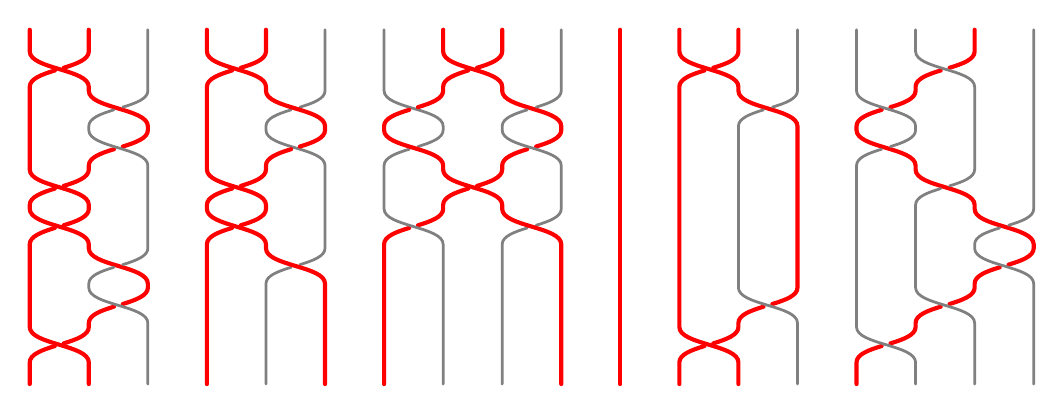
\begin{tikzpicture}
  \pic[
    line width=1.5pt,
    red,
    line cap=round,
    braid/.cd,
    width=.75cm,
    crossing height=.5cm,
    strand 3/.style={gray,line width=1pt},
    strand 6/.style={gray,line width=1pt},
    strand 7/.style={gray,line width=1pt},
    strand 10/.style={gray,line width=1pt},
    strand 14/.style={gray,line width=1pt},
    strand 15/.style={gray,line width=1pt},
    strand 16/.style={gray,line width=1pt},
    strand 18/.style={gray,line width=1pt},
  ] {braid={s_1-s_4-s_8-s_{12}-s_{16} s_2-s_5-s_7-s_9-s_{13}-s_{15} s_2-s_5-s_7-s_9-s_{15} s_1-s_4-s_8-s_{16} s_1-s_4-s_7-s_9-s_{17} s_2-s_5-s_{17} s_2-s_{13}-s_{16} s_1-s_{12}-s_{15}}};
\end{tikzpicture}
\end{center}

\section{Introduction}

This is a package for drawing braid diagrams using PGF/TikZ.
An example follows.

\begin{example}
\begin{center}
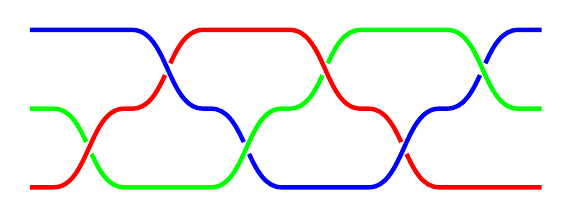
\begin{tikzpicture}
\pic[
  rotate=90,
  braid/.cd,
  every strand/.style={ultra thick},
  strand 1/.style={red},
  strand 2/.style={green},
  strand 3/.style={blue},
] {braid={s_1 s_2^{-1} s_1 s_2^{-1} s_1 s_2^{-1}}};
\end{tikzpicture}
\end{center}
\end{example}

This is actually the documentation for two packages: a \emph{package} and a TikZ \emph{library}.
If your preamble contains \Verb+\usepackage{braids}+ then you are using the package, if \Verb+\usetikzlibrary{braids}+ then the library.

The package was the original version, and then with the advent of \Verb+pic+s I rewrote it as a TikZ library.
If you are starting afresh then you should use the library, but I recognise that people might have figured out how to get what they want with the old package and don't need to switch.
So although the original package should be considered \emph{depreciated}, it is not (yet) obsolete.
I will continue to fix bugs for the original package, but new features only go in the TikZ library.

\section{TikZ Library Usage}

Version 2.0 changed the implementation to use the TikZ \Verb+pic+ syntax.
It also converted it to a TikZ library, so to use it put the following in the preamble.

\begin{verbatim}
\usetikzlibrary{braids}
\end{verbatim}

(Or add it to the copious list of TikZ libraries that you are already using.)

\bigskip

\DescribeMacro{braid}
A braid is specified by the pic name \Verb+braid+.
The usual syntax for this is as follows:

\Verb+\pic[options] at (coordinate) {braid={braid-word}};+

\DescribeMacro{braid-word}
The \Verb+braid-word+ is an expression in the braid group, such as \Verb+s_1 s_2^{-1} s_{3,5}+.
The generator labels are not significant.

The subscript determines how the strands cross, as follows:
\begin{enumerate}
\item If the subscript is a single number, as in \Verb+s_2+, the crossing goes from that number over the next.
\item If the subscript is two or more numbers separated by a comma, as in \Verb+s_{2,4}+ or \Verb+s_{1,3,5}+, imagine holding the numbered strands and moving each to the position of the next with the last strand moving under the others to where the first stands.
Any intermediate non-specified strand is behind all those involved in the crossing.
\item If the subscript is hyphenated, as in \Verb+s_{1-5}+, this is equivalent to \Verb+s_{1,2,3,4,5}+.
This can be used as part of a list, as in \Verb+s_{1-3,5}+.
\end{enumerate}

All of these crossings take place in the same amount of vertical space.
Be advised that crossings involving a lot of strands can get quite squashed.

The exponent can be \Verb+1+, \Verb+{-1}+, or missing (in which case it defaults to \Verb+1+, note also that the exponent is read as a \TeX-token so \Verb+{1}+ is also legal).
If the exponent is \(-1\) then the braid element represented by the crossing is inverted.

\begin{itemize}
\item \Verb+s_1+ is strand \(1\) over strand \(2\).
\item \Verb+s_1^{-1}+ is strand \(2\) over strand \(1\).
\item \Verb+s_{1,3}+ is strand \(1\) over strand \(3\), and both are over strand \(2\).
\item \Verb+s_{1-3}+ is strand \(3\) under strand \(2\) and then under strand \(1\).
\end{itemize}

Certain other symbols are allowed in the \Verb+braid-word+ which control the rendering of the braid.
These extras are as follows.

\begin{enumerate}
\item To get crossings to render at the same height, separate them with a hyphen (note: no check is made to ensure that the crossings can legally be put at the same height; \emph{caveat emptor}).
For example, \Verb+s_1-s_3+.

\item To draw a \emph{floor} -- which is a rectangle behind the braid occupying some number of levels (the default being one level) -- precede the braid element by a vertical line, as in \Verb+s_1 | s_2+.
The floor is itself a pic which, by default, consists of a rectangle and two horizontal lines.
The rectangle picks up any \Verb+fill+ options and the lines any \Verb+draw+ options that are set in the \Verb+braid/every floor+ and \Verb+braid/floor <n>+ styles, which are documented below (with an example of changing the pic).
The \Verb+n+ is the level number, starting at \(1\).

More general floors can be drawn using the key \Verb+braid/add floor+.
This takes one argument which is a comma separated list of parameters that specifies the position and size floor:
%
\begin{verbatim}
braid/add floor={x,y,width,height,name}
\end{verbatim}
%
The units used are the ``natural'' units of the braid: strand separation and level height.
The \Verb+name+ is optional and if given can be used to style the floor in that the style \Verb+braid/floor <name>+ is applied to that floor.

Replacing the floor pic will change how it is drawn.
The coordinate system is set up for the floor pic so that the floor is a unit square with lower left corner at the origin.
The default definition is:

\begin{lstlisting}
  floor/.pic={
    \path[pic actions, draw=none] (0,0) rectangle (1,1);
    \path[pic actions, fill=none] (0,0) -- (1,0) (0,1) -- (1,1);
  }
\end{lstlisting}

\item The identity element can occur in the braid-word.
It is represented by \Verb+1+.
This inserts the identity which corresponds to no crossing.
However, it takes the same amount of space as if there were a crossing.

\end{enumerate}

\subsection{Style Options}
\label{sec:picstyleopts}

There are various keys that change the behaviour or rendering of the braid.
All of these are in the \Verb+/tikz/braid/+ namespace.
Many of the examples use the key \Verb+braid/.cd+ to switch to this namespace, meaning that multiple \Verb+braid+ keys can be given without the \Verb+braid+ prefix.
Any unknown keys are dropped back to the \Verb+tikz+ namespace.
See the TikZ/pgf documentation for more details on key handling.

\DescribeMacro{number of strands} The key \Verb+number of strands+ sets the minimum number of strands for the braid.
The number of strands will grow according to the terms in the braid word so this merely sets a lower bound.
If not set, the number of strands will be determined by the terms in the braid word.

\DescribeMacro{height}
The key \Verb+height+ is used to set the height of the piece of the braid corresponding to a single element in the group.
This can be negative, and indeed the default value is negative because the default is for a braid to flow down the page.

This key is depreciated and is only kept for backwards compatibility, the fact that the default is negative proved confusing.
Therefore the following key should be used in its place.

\DescribeMacro{crossing height}
The key \Verb+crossing height+ also sets the height of the piece of the braid corresponding to an element in the group.
The sign of this is ignored.

The correct way to get a braid to flow in a different direction to the default is to use a transformation on the \Verb+pic+, such as in the following example.

\begin{example}
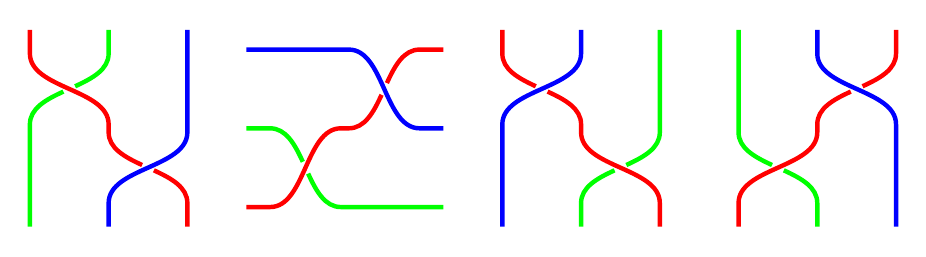
\begin{tikzpicture}[
  every braid/.style={
    ultra thick,
    braid/strand 1/.style=red,
    braid/strand 2/.style=green,
    braid/strand 3/.style=blue,
    braid/anchor=center,
    }
  ]
\pic {braid={s_1 s_2^{-1}}};
\pic[rotate=90] at (3,0) {braid={s_1 s_2^{-1}}};
\pic[rotate=180] at (6,0) {braid={s_1 s_2^{-1}}};
\pic[yscale=-1] at (9,0) {braid={s_1 s_2^{-1}}};
\end{tikzpicture}
\end{example}

The \Verb+crossing height+ and \Verb+height+ keys shouldn't be used together.
If they are then a message will be printed on the console and the value for \Verb+crossing height+ will be used.

\DescribeMacro{width}
The key \Verb+width+ sets the separation of the strands in the braid.
This can be negative.

\DescribeMacro{border height}
The key \Verb+border height+ adds a little extra length to the strands at the start and end of the braid.

\DescribeMacro{gap}
The key \Verb+gap+ is used to determine how much of a gap to leave in the under strand at a crossing.
This should be a number strictly between 0 and .5.
The curve is drawn using a cubic b\'ezier and the gap is in terms of the time parameter, so the gap will not increase exactly proportionally to the value given by this key, though that is a reasonable approximation.

\DescribeMacro{control factor}
As just said, the parts of the strands involved in a crossing are drawn using a cubic b\'ezier curve.
The control points are vertically above or below their respective end point.
This key determines that vertical separation.
It is multiplied by the \Verb+height+ so that it scales properly.
It can be set to 0 whereupon the strands in the crossing are straight lines.
The default is 0.5.

\DescribeMacro{nudge factor}
The crossings are not quite placed one after another.
There is a small ``nudge'' between the end of one crossing and the start of another.
Due to the way that the strands are lengthened, if there is no ``nudge'' then some PDF renderers produce slightly strange results at certain magnifications.
This key controls how much that ``nudge'' is, as a factor of the \Verb+height+.
For the aforementioned reason, it should not be set to 0 (the default is 0.05).
Note that this does not change the height of a crossing.
Rather, it nudges the height at which the strands start to cross over.

\DescribeMacro{every braid}
This style is invoked on a scope that surrounds the actual braid.
It can be used to set defaults for a group of braids.

\DescribeMacro{every strand, strand <n>}
The style of the strands are controlled by two types of option.
Style options that are set on the \Verb+pic+ are passed to every strand.
It is also possible to add style options to individual strands using the keys \Verb+every strand+ and \Verb+strand <n>+.
The strands are numbered by their starting position.

\DescribeMacro{every floor, floor <n>}
When a floor is requested behind a crossing, it is rendered as a pic.
These keys control how the floor is styled.
They can even be used to change the \Verb+pic+ used to draw individual floors.
The \Verb+n+ is the level number, starting at \(1\).

\begin{example}
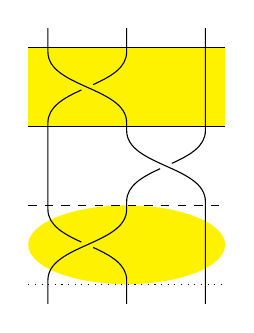
\begin{tikzpicture}
\pic[
  braid/floor 3/.style={
    floor/.pic={
      \path[pic actions, draw=none] (.5,.5) circle[x radius=.5, y radius=.5];
      \path[pic actions, fill=none, dashed] (0,0) -- (1,0);
      \path[pic actions, fill=none, dotted] (0,1) -- (1,1);
    },
  },
  braid/every floor/.style={
    fill=yellow,
    draw=black
  }
] {braid={| s_1 s_2 | s_1^{-1}}};
\end{tikzpicture}
\end{example}

\subsection{Coordinates and Anchors}

The braid is littered with coordinates.
Each strand gets a coordinate at each end, and at every level between crossings.
These are labelled and numbered by the initial strand position and the crossing level.
They are also labelled and numbered by the final strand position with the prefix \Verb+rev+.
If the braid has been named, the coordinate names look like the following:
%
\begin{lstlisting}
  <braid name>-<strand number>-<crossing number>
  <braid name>-rev-<strand number>-<crossing number>
\end{lstlisting}
%
The crossing number can also be either \Verb+s+ or \Verb+e+ for the start and end of the strand.
Note that \Verb+-1-0+ and \Verb+-1-s+ are slightly different in that \Verb+s+ includes the border height.

In addition, if the braid is named then a rectangular node is defined that fits around the whole braid.
This node is not defined in the standard way, so -- for example -- it can't directly be used to draw a border, but TikZ behaves afterwards as if it were.
In particular its anchors can be used to define locations around the edge of the braid.

\begin{example}
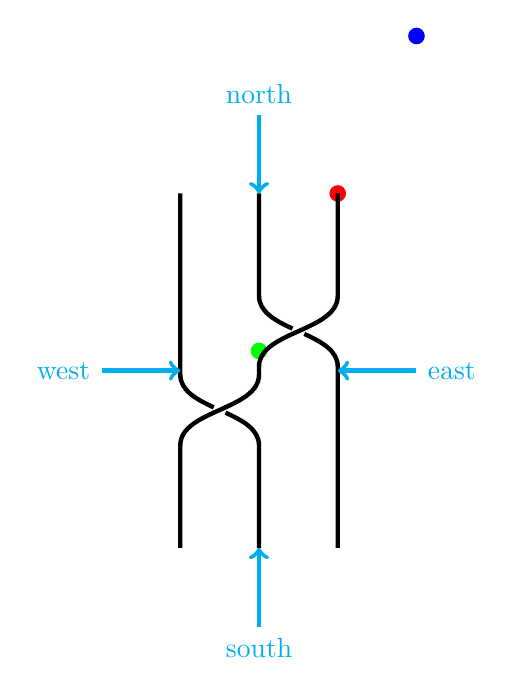
\begin{tikzpicture}[ultra thick]
\fill[red] (1,2) circle[radius=3pt];
\fill[blue] (2,4) circle[radius=3pt];
\fill[green] (0,0) circle[radius=3pt];
\pic[
  braid/.cd,
  crossing height=-1cm,
  width=-1cm,
  anchor=north east,
] (anchors) at (1,2) {braid={1 s_1 s_2 1}};
\draw[<-,cyan] (anchors.east) -- +(1,0) node[right] {east};
\draw[<-,cyan] (anchors.west) -- +(-1,0) node[left] {west};
\draw[<-,cyan] (anchors.north) -- +(0,1) node[above] {north};
\draw[<-,cyan] (anchors.south) -- +(0,-1) node[below] {south};
\end{tikzpicture}
\end{example}

\DescribeMacro{anchor}
The key \Verb+anchor+ (in the \Verb+braid+ name space) can be used to shift the braid so that a different part of it is at the specified location.
If the argument contains a hyphen then it is assumed to refer to a point on a strand with the same interpretation as the coordinates.
If the argument does not contain a hyphen then it is taken to be an anchor of a surrounding rectangular node (the node might not itself exist -- if the braid isn't named -- but that doesn't affect the positioning).
In the following example, the braid is shifted so that where the third strand starts the second level is at the position \Verb+(1,1)+

\begin{example}
\begin{center}
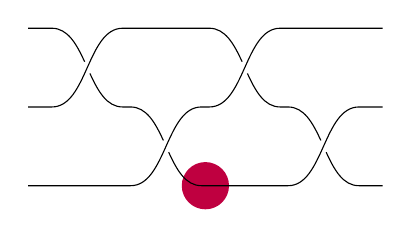
\begin{tikzpicture}
\fill[purple] (1,1) circle[radius=3mm];
\pic[braid/anchor=3-2,rotate=90] at (1,1) {braid={s_2 s_1 s_2 s_1}};
\end{tikzpicture}
\end{center}
\end{example}


\subsection{Examples}

Here are more detailed examples.

\begin{example}
\begin{center}
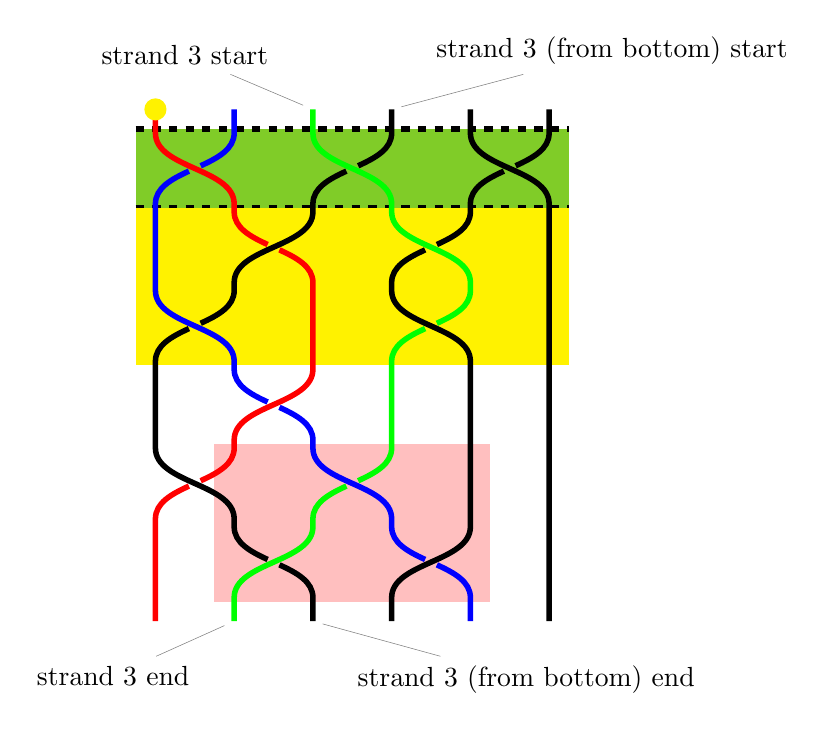
\begin{tikzpicture}
\pic[
  braid/every floor/.style={fill=yellow},
  braid/floor 1/.style={draw=black,dashed,fill=yellow!50!green},
  line width=2pt,
  braid/strand 1/.style={red},
  braid/strand 2/.style={blue},
  braid/strand 3/.style={green},
  braid/add floor={2,4,3,2,a},
  braid/floor a/.style={fill=pink},
  name=coordinates,
] at (2,0) {braid={| s_1-s_3-s_5 | s_2^{-1}-s_4| s_1-s_4 s_2^{-1} s_1-s_3 s_2^{-1}-s_4^{-1}}};
\fill[yellow] (2,0) circle (4pt);
\node[at=(coordinates-3-s),pin=north west:strand 3 start] {};
\node[at=(coordinates-3-e),pin=south west:strand 3 end] {};
\node[at=(coordinates-rev-3-s),pin=north east:strand 3 (from bottom) start] {};
\node[at=(coordinates-rev-3-e),pin=south east:strand 3 (from bottom) end] {};
\end{tikzpicture}
\end{center}
\end{example}

\begin{example}
\begin{center}
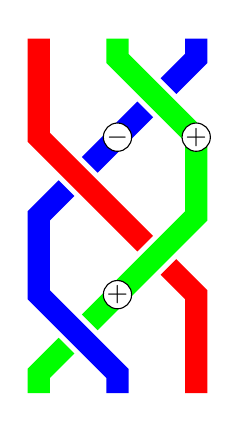
\begin{tikzpicture}
\pic[
  braid/.cd,
  number of strands=3,
  line width=8pt,
  strand 1/.style={red},
  strand 2/.style={green},
  strand 3/.style={blue},
  gap=0.1,
  control factor=0,
  nudge factor=0,
  name=symbols,
] {braid={a_2 a_1 a_2^{-1} a_1}};
\node[circle,draw,fill=white,inner sep=0pt] at (symbols-2-1) {\(+\)};
\node[circle,draw,fill=white,inner sep=0pt] at (symbols-3-1) {\(-\)};
\node[circle,draw,fill=white,inner sep=0pt] at (symbols-2-3) {\(+\)};
\end{tikzpicture}
\end{center}

\end{example}

\begin{example}
\begin{center}
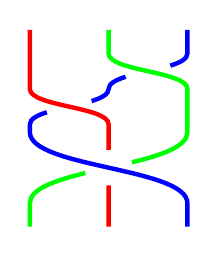
\begin{tikzpicture}
\pic[
  braid/.cd,
  number of strands=3,
  ultra thick,
  strand 1/.style={red},
  strand 2/.style={green},
  strand 3/.style={blue},
  gap=0.1,
] {braid={a_{1-3} a_{1,3}}};
\end{tikzpicture}
\end{center}

\end{example}

The next example uses the nonlinear transformations pgf module with the following definition.

\begin{lstlisting}
  \usepgfmodule{nonlineartransformations}
  \makeatletter
  \def\polartransformation{%
    % \pgf@x will contain the radius
    % \pgf@y will contain the distance
    \pgfmathsincos@{\pgf@sys@tonumber\pgf@x}%
    % pgfmathresultx is now the cosine of radius and
    % pgfmathresulty is the sine of radius
    \pgf@x=\pgfmathresultx\pgf@y%
    \pgf@y=\pgfmathresulty\pgf@y%
  }
  \makeatother
\end{lstlisting}

\begin{example}
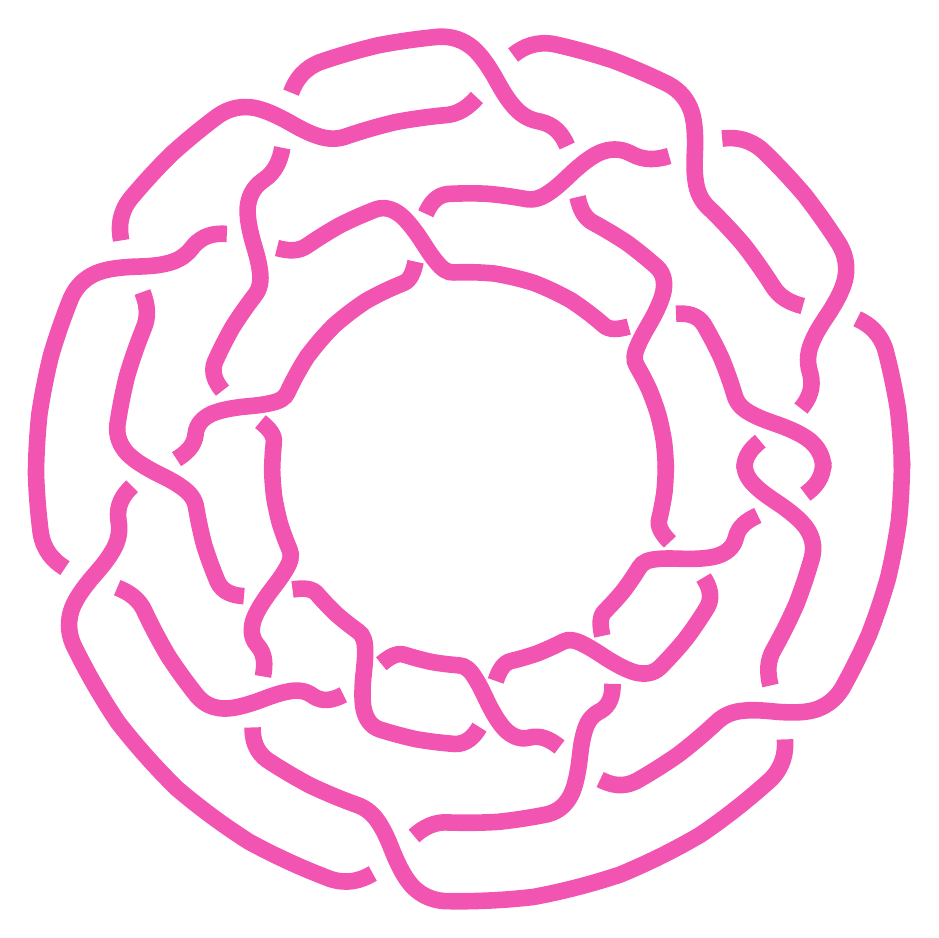
\begin{tikzpicture}[scale=.5]
\begin{scope}
\pgftransformnonlinear{\polartransformation}% see above
\pic[
  rotate=90,
  braid/.cd,
  every strand/.style={line width=6pt,magenta!67},
  border height=0cm,
  crossing height=15.7pt,
  gap=.2,
  nudge factor=0.01,
] at (0,5) {braid=%
  s_2^{-1} s_3 s_1 s_3 s_2^{-1} s_3 s_1 s_3
  s_2^{-1} s_3 s_1 s_2^{-1} s_3 s_1 s_2^{-1}
  s_1 s_3 s_1 s_2^{-1} s_1 s_3 s_1 s_2^{-1}
};
\end{scope}

\end{tikzpicture}
\end{example}

\newpage

Here's an example using a decoration library to style the strands.

\begin{justexample}

\begin{tikzpicture}[remember picture, overlay]
\pic[
  decoration={
    markings,
    mark=between positions 2mm and 1 step 5mm with {
      \draw[black,thick] (-2mm,-1.5mm) .. controls +(4mm,0) and +(-4mm,0) .. (2mm,1.5mm);
    }
  },
  braid/number of strands=10,
  braid/gap=.15,
  braid/every strand/.style={
    line width=3mm,
    draw,
    brown!50,
    postaction={
      decorate,
    },
    preaction={
      draw,
      black,
      line width=3.3mm,
    }
  },
  braid/every floor/.style={
    draw
  },
  braid/height=-3cm,
  braid/width=2cm,
  braid/anchor=1-0,
]
at ([shift={(2,-2)}]current page.north west)
{braid={
    s_1-s_3-s_5^{-1}-s_7^{-1}
    s_1-s_3-s_5^{-1}-s_7^{-1}
    s_1-s_3-s_5^{-1}-s_7^{-1}
    s_1-s_3-s_5^{-1}-s_7^{-1}
    s_1-s_3-s_5^{-1}-s_7^{-1}
    s_1-s_3-s_5^{-1}-s_7^{-1}
    s_1-s_3-s_5^{-1}-s_7^{-1}
    s_1-s_3-s_5^{-1}-s_7^{-1}
}};
\begin{scope}[shift={([shift={(1,-2)}]current page.north west)}]
\draw (0,0) grid[xstep=4cm,ystep=3cm] ++(20,-24.1);
\draw (18,0) -- +(0,-24.1);
\end{scope}
\end{tikzpicture}
\end{justexample}

\newpage


\begin{tikzpicture}[remember picture, overlay]
\pic[
  decoration={
    markings,
    mark=between positions 2mm and 1 step 5mm with {
      \draw[black,thick] (-2mm,-1.5mm) .. controls +(4mm,0) and +(-4mm,0) .. (2mm,1.5mm);
    }
  },
  braid/number of strands=10,
  braid/gap=.15,
  braid/every strand/.style={
    line width=3mm,
    draw,
    brown!50,
    postaction={
      decorate,
    },
    preaction={
      draw,
      black,
      line width=3.3mm,
    }
  },
  braid/every floor/.style={
    draw
  },
  braid/height=-3cm,
  braid/width=2cm,
  braid/anchor=1-0,
]
at ([shift={(2,-2)}]current page.north west)
{braid={
    s_1-s_3-s_5^{-1}-s_7^{-1}
    s_1-s_3-s_5^{-1}-s_7^{-1}
    s_1-s_3-s_5^{-1}-s_7^{-1}
    s_1-s_3-s_5^{-1}-s_7^{-1}
    s_1-s_3-s_5^{-1}-s_7^{-1}
    s_1-s_3-s_5^{-1}-s_7^{-1}
    s_1-s_3-s_5^{-1}-s_7^{-1}
    s_1-s_3-s_5^{-1}-s_7^{-1}
}};
\begin{scope}[shift={([shift={(1,-2)}]current page.north west)}]
\draw (0,0) grid[xstep=4cm,ystep=3cm] ++(20,-24.1);
\draw (18,0) -- +(0,-24.1);
\end{scope}
\end{tikzpicture}

\newpage

\section{Original Package Usage (Depreciated)}

The original version was as a separate package.
This is still included for backwards compatibility.
To use this package, you need to put the following in the preamble.

\begin{verbatim}
\usepackage{braids}
\end{verbatim}

\DescribeMacro{\braid}
A braid is specified by the command \Verb+\braid+.
The syntax for this command is as follows:

\Verb+\braid[style options] (name) at (coordinate) braid-word;+

\DescribeMacro{braid-word}
The \Verb+braid-word+ is an expression in the braid group, such as \Verb+s_1 s_2^{-1}+.
The generator labels are not significant.
The exponent can be \Verb+1+, \Verb+{-1}+, or missing (in which case it defaults to \Verb+1+, note also that the exponent is read as a \TeX-token so \Verb+{1}+ is also legal).
Certain other symbols are allowed in the \Verb+braid-word+ which control the rendering of the braid.
These extras are as follows.

\begin{enumerate}
\item To get crossings to render at the same height, separate them with a hyphen (note: no check is made to ensure that the crossings can legally be put at the same height; \emph{caveat emptor}).

\item To draw a \emph{floor}, precede the braid element by a vertical line.
What happens then is that when the braid is rendered, the coordinates of the rectangle behind that crossing (wide enough to encompass all the strands) is passed to a command.
The intention is that this command draw something behind the braid.
The command is configurable by a key (see \ref{sec:styleopts}).

\item The identity element can occur in the braid-word.
It is represented by \Verb+1+.
This inserts the identity which corresponds to no crossing.
However, it takes the same amount of space as if there were a crossing.

\item Strands can be labelled between crossings.
To do this, the commands \Verb+\label+, \Verb+\olabel+, and \Verb+\clabel+ are provided.
These take three arguments, the first is optional.
The result of this command is to place a node on top of a particular strand between the crossings where the command is given.
The first (optional) argument can be used to pass style options to this node.
The second argument is the strand number.
The third argument is the label text.

The three commands differ as to how they interpret the strand number.
For \Verb+\olabel+, the strand number is taken to mean the strand that starts at that position.
For \Verb+\clabel+, the strand number is taken to mean the strand that is currently at that position.
The behaviour of \Verb+\label+ is to choose one or other of these depending on whether the key \Verb+strand label by origin+ is true or false.
This key only has an effect at the start of the braid-word; it cannot be reset in the middle.

\item Style options can be given in the middle of a braid-word by enclosing them in square brackets.
There are not many style options that it makes sense to change in the middle of the braid-word, since the strands are rendered all in one go at the end.

\item Scoping is handled by using braces.
Thus to change a style only briefly, enclose the desired scope in braces.
\end{enumerate}

\DescribeMacro{name}
The (optional) \Verb+name+ acts a little like the \Verb+name+ of a TikZ node.
When it is specified, the routine that renders the braid also saves certain coordinates as if they were node anchors.
Specifically, \Verb+coordinate+ nodes are placed at the centre of the braid diagram and at the ends of each strand.
The centre has the label \Verb+name+, the strands are labelled \Verb+name-number-end+ and \Verb+name-rev-number-end+, where \Verb+name+ is the name given to the braid, \Verb+number+ is the number of the strand counting from the left, and \Verb+end+ is either \Verb+s+ for the start or \Verb+e+ for the end.
If the version with \Verb+rev+ is used then the numbers correspond to the \emph{final} positions of the braids.
The name can also be specified with the \Verb+name+ key.

\DescribeMacro{at}
The (optional) \Verb+at (coordinate)+ syntax positions the braid at the \Verb+coordinate+ in the current picture.
Due to the implementation, the coordinate has to be known at the start, but the width and height of the braid are only known at the end.
Therefore, the braid is positioned so that the start of the first strand is at \Verb+(coordinate)+.
This can also be specified using the \Verb+at+ key.

\DescribeMacro{style options}
The \Verb+style options+ set the style for the braid strands.
They can be grouped into three types: options that set up the main parameters for the braid, options that set the default style for the strands, and options that set up styles for individual strands.
The options are as follows.

\subsection{Style Options}
\label{sec:styleopts}

\DescribeMacro{number of strands} The key \Verb+number of strands+ sets the minimum number of strands for the braid.
The number of strands will grow according to the terms in the braid word so this merely sets a lower bound.
If not set, the number of strands will be determined by the terms in the braid word.

\DescribeMacro{height}
The key \Verb+height+ sets the height of the piece of the braid corresponding to an element in the group.

\DescribeMacro{width}
The key \Verb+width+ sets the separation of the strands in the braid.

\DescribeMacro{border height}
The key \Verb+border height+ adds a little extra length to the strands at the start and end of the braid.

\DescribeMacro{gap}
The key \Verb+gap+ is used to determine how much of a gap to leave in the under strand at a crossing.
This should be a number strictly between 0 and .5.
The curve is drawn using a cubic b\'ezier and the gap is in terms of the time parameter, so the gap will not increase exactly proportionally to the value given by this key, though that is a reasonable approximation.

\DescribeMacro{control factor}
As just said, the parts of the strands involved in a crossing are drawn using a cubic b\'ezier curve.
The control points are vertically above or below their respective end point.
This key determines that vertical separation.
It is multiplied by the \Verb+height+ so that it scales properly.
It can be set to 0 whereupon the strands in the crossing are straight lines.
The default is 0.5.

\DescribeMacro{nudge factor}
The crossings are not quite placed one after another.
There is a small ``nudge'' between the end of one crossing and the start of another.
Due to the way that the strands are lengthened, if there is no ``nudge'' then some PDF renderers produce slightly strange results at certain magnifications.
This key controls how much that ``nudge'' is, as a factor of the \Verb+height+.
For the aforementioned reason, it should not be set to 0 (the default is 0.05).
Note that this does not change the height of a crossing.
Rather, it nudges the height at which the strands start to cross over.

\DescribeMacro{style strands}
The style of the strands are controlled by two types of option.
Style options that are set on the \Verb+\braid+ command are passed to every strand.
It is also possible to add style options to individual strands using the key \Verb+style strands+.
This takes two options, a comma-delimited list of strand numbers (which could be just a single number) and a list of options to be applied to that strand.
Thus, the syntax is \Verb+style strands={n,m,...}{options}+.
The strands are numbered by their starting position.
Not all of the standard TikZ style options are possible due to the way that the strands are constructed.
Basically, the options that are allowed are those that do not require changing the path or drawing it more than once.

\DescribeMacro{floor command}
When a floor is requested behind a crossing, the actual way to render it is determined by a command.
This key allows the user to define that command.
The argument to this key should be the code that should be executed for each floor.
To avoid the hassle of getting the number of hashes right, the command should take no arguments.
Rather, the coordinates of the rectangle are saved in to macros \Verb+\floorsx+, \Verb+\floorsy+, \Verb+\floorex+, \Verb+\floorey+ (these macros will expand to something like \Verb+10pt+) and the command should use these to position the drawing.
The default is to draw a line at the top and at the bottom of the rectangle.

\DescribeMacro{style floors}
\DescribeMacro{style all floors}
In the spirit of separating \emph{style} and \emph{content}, the style options for the floors can be specified separately to the command (of course, they could be built in to the command).
One advantage of this over building them in to the command is to allow them to be overridden for individual floors.
The \Verb+style all floors+ sets up options to be used for \emph{all} floors, whilst the \Verb+style floors={n,m,...}{options}+ sets up options to be used only for the listed floor.
Anything specified in the \Verb+floor command+ will take precedence over both of these.

Any other style options are passed to the underlying TikZ/PGF system and so may influence how the braid is drawn (but note that not all keys make sense due to the implementation).


\subsection{Examples}

Here are more detailed examples.

\begin{example}
\begin{center}
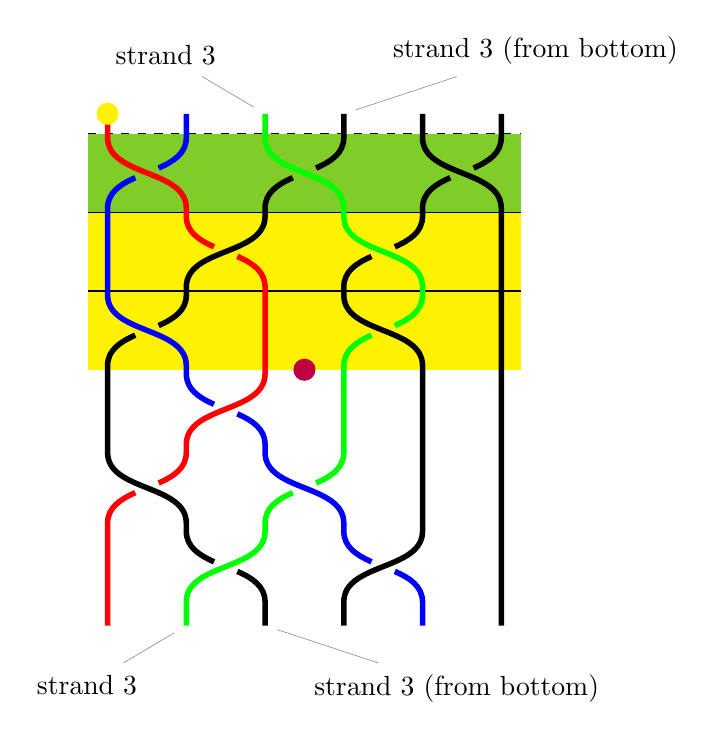
\begin{tikzpicture}
\braid[
  style all floors={fill=yellow},
  style floors={1}{dashed,fill=yellow!50!green},
  floor command={%
   \fill (\floorsx,\floorsy) rectangle (\floorex,\floorey);
   \draw (\floorsx,\floorsy) -- (\floorex,\floorsy);
  },
  line width=2pt,
  style strands={1}{red},
  style strands={2}{blue},
  style strands={3}{green}
] (strands) at (2,0) | s_1-s_3-s_5 | s_2^{-1}-s_4| s_1-s_4 s_2^{-1} s_1-s_3 s_2^{-1}-s_4^{-1};
\fill[yellow] (2,0) circle (4pt);
\fill[purple] (strands) circle (4pt);
\node[at=(strands-3-s),pin=north west:strand 3] {};
\node[at=(strands-3-e),pin=south west:strand 3] {};
\node[at=(strands-rev-3-s),pin=north east:strand 3 (from bottom)] {};
\node[at=(strands-rev-3-e),pin=south east:strand 3 (from bottom)] {};
\end{tikzpicture}
\end{center}
\end{example}

\begin{example}
\begin{center}
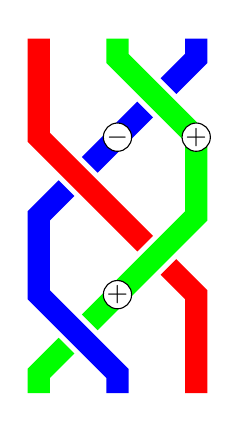
\begin{tikzpicture}
\braid[
  number of strands=3,
  line width=8pt,
  style strands={1}{red},
  style strands={2}{green},
  style strands={3}{blue},
  gap=0.1,
  control factor=0,
  nudge factor=0,
  strand label by origin=true,
  strand label/.style={circle,draw,fill=white,inner sep=0pt},
  yscale=1] (braid_1) a_2 \label{2}{\(+\)} \clabel{2}{\(-\)} a_1 a_2^{-1} \olabel{2}{\(+\)} a_1;
\end{tikzpicture}
\end{center}

\end{example}

\end{document}
% Local Variables:
% tex-output-type: "pdf18"
% End:
